\section{Results} % (fold)
\label{sec:results}

\subsection{Choosing the board} % (fold)
\label{sub:choosing_the_board}
In order to analyse the behavior of the game in various situations,
we decided to define four boards that globally represent the possible
distributions of traps on the board. They are defined as
\begin{enumerate}
  \item A \emph{uniformly low} density trap-distributed board,
  \item a \emph{left high} density trap-distributed board,
  \item a \emph{right high} density trap-distributed board,
  \item and a \emph{uniformly high} density trap-distributed board.
\end{enumerate}
The results presented in this section will correspond to the first case,
as it is likely to represent most of real life \emph{Snake and Ladder} games.
However, appendix~\ref{app:additional_error_plots} will contain the results
of the three other board distributions and some comment on them will be
made at the end of this section.

\todo{Generate the figure/results for those cases (in appendix?) with boards defined
in experiments.jl OR remove this section.}

Figure~\ref{fig:board_unif_low} represents the board we used to conduct the experiments.

\begin{figure}[H]
\centering
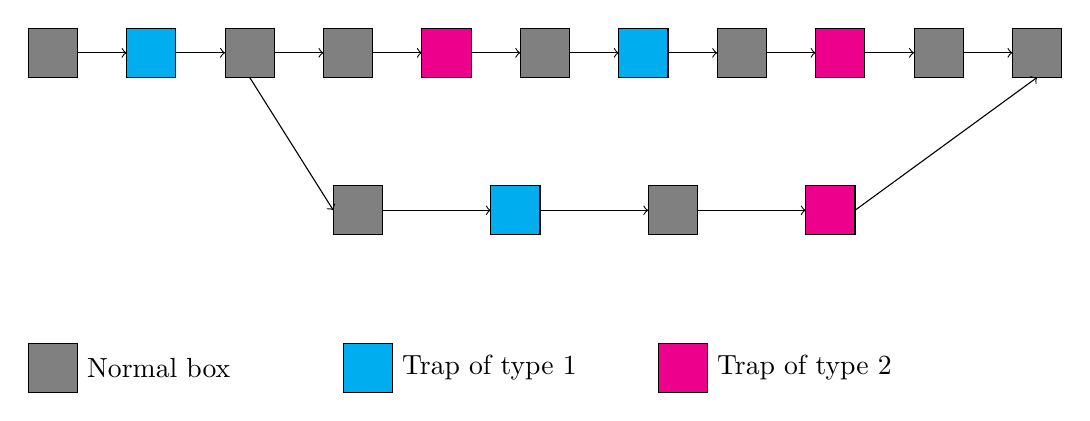
\begin{tikzpicture}[scale=10]
%board = [0,1,0,0,2,0,1,0,2,0,0,1,0,2,0]
\pgfmathsetmacro{\i}{1-1}
\pgfmathsetmacro{\c}{"gray"}
\draw [fill=\c] (2*\i*0.0625,1) rectangle (2*\i*0.0625+0.0625,1-0.0625);
\pgfmathsetmacro{\i}{2-1}
\pgfmathsetmacro{\c}{"cyan"}
\draw [fill=\c] (2*\i*0.0625,1) rectangle (2*\i*0.0625+0.0625,1-0.0625);
\pgfmathsetmacro{\i}{3-1}
\pgfmathsetmacro{\c}{"gray"}
\draw [fill=\c] (2*\i*0.0625,1) rectangle (2*\i*0.0625+0.0625,1-0.0625);
\pgfmathsetmacro{\i}{4-1}
\pgfmathsetmacro{\c}{"gray"}
\draw [fill=\c] (2*\i*0.0625,1) rectangle (2*\i*0.0625+0.0625,1-0.0625);
\pgfmathsetmacro{\i}{5-1}
\pgfmathsetmacro{\c}{"magenta"}
\draw [fill=\c] (2*\i*0.0625,1) rectangle (2*\i*0.0625+0.0625,1-0.0625);
\pgfmathsetmacro{\i}{6-1}
\pgfmathsetmacro{\c}{"gray"}
\draw [fill=\c] (2*\i*0.0625,1) rectangle (2*\i*0.0625+0.0625,1-0.0625);
\pgfmathsetmacro{\i}{7-1}
\pgfmathsetmacro{\c}{"cyan"}
\draw [fill=\c] (2*\i*0.0625,1) rectangle (2*\i*0.0625+0.0625,1-0.0625);
\pgfmathsetmacro{\i}{8-1}
\pgfmathsetmacro{\c}{"gray"}
\draw [fill=\c] (2*\i*0.0625,1) rectangle (2*\i*0.0625+0.0625,1-0.0625);
\pgfmathsetmacro{\i}{9-1}
\pgfmathsetmacro{\c}{"magenta"}
\draw [fill=\c] (2*\i*0.0625,1) rectangle (2*\i*0.0625+0.0625,1-0.0625);
\pgfmathsetmacro{\i}{10-1}
\pgfmathsetmacro{\c}{"gray"}
\draw [fill=\c] (2*\i*0.0625,1) rectangle (2*\i*0.0625+0.0625,1-0.0625);
\pgfmathsetmacro{\i}{11-11}
\pgfmathsetmacro{\c}{"gray"}
\draw [fill=\c] (0.45+\i*0.2,0.8) rectangle (0.45+\i*0.2-0.0625,0.8-0.0625);
\pgfmathsetmacro{\i}{12-11}
\pgfmathsetmacro{\c}{"cyan"}
\draw [fill=\c] (0.45+\i*0.2,0.8) rectangle (0.45+\i*0.2-0.0625,0.8-0.0625);
\pgfmathsetmacro{\i}{13-11}
\pgfmathsetmacro{\c}{"gray"}
\draw [fill=\c] (0.45+\i*0.2,0.8) rectangle (0.45+\i*0.2-0.0625,0.8-0.0625);
\pgfmathsetmacro{\i}{14-11}
\pgfmathsetmacro{\c}{"magenta"}
\draw [fill=\c] (0.45+\i*0.2,0.8) rectangle (0.45+\i*0.2-0.0625,0.8-0.0625);
\pgfmathsetmacro{\i}{15-5}
\pgfmathsetmacro{\c}{"gray"}
\draw [fill=\c] (2*\i*0.0625,1) rectangle (2*\i*0.0625+0.0625,1-0.0625);

\foreach \i in {0,1,...,9}
	\draw [->] (0.0625+2*\i*0.0625,1-0.03125) -- (2*0.0625+2*\i*0.0625,1-0.03125);
\foreach \i in {0,1,2}
	\draw [->] (0.45+\i*0.2,0.8-0.03125) -- (0.45+0.1375+\i*0.2,0.8-0.03125);
\draw [->] (5*0.0625-0.03125,1-0.0625) -- (0.45-0.0625, 0.8-0.03125);
\draw [->] (0.45+0.1375+2*0.2+0.0625,0.8-0.03125) -- (2*10*0.0625+0.0625/2,1-0.0625);

\draw [fill=gray] (0,0.6) rectangle (0.0625, 0.6-0.0625);
\node [right] at (0.0625, 0.6-0.03125) {Normal box};
\draw [fill=cyan] (0.4,0.6) rectangle (0.4 + 0.0625, 0.6-0.0625);
\node [right] at (0.4 + 0.0625, 0.6-0.03125) {Trap of type 1};
\draw [fill=magenta] (0.8,0.6) rectangle (0.8 + 0.0625, 0.6-0.0625);
\node [right] at (0.8 + 0.0625, 0.6-0.03125) {Trap of type 2};
\end{tikzpicture}
\caption{Representation of our board.}
\label{fig:board_unif_low}
\end{figure}
% subsection choosing_the_board (end)

\subsection{Design of the experiments}
Given a particular board configuration, we executed the following three types of experiments : 
\begin{enumerate}
	\item Comparison of simulated and expected cost starting from box 1.
	The simulated cost is the average cost obtained ater a certain number of simulations.
	It is computed for a number of simulations that varies between $10$ and $10^7$. 
	The evolution of this cost is then plotted together with the expected cost obtained by value-iteration.
	\item Comparison of simulated and expected cost starting from each box for a fixed number of simulations.
	\item Comparison of simulated cost using the optimal strategy and some sub-optimal strategies. 
	Here, the evolution of the average cost  with the number of simulations are displayed for each strategy on the same graph.
\end{enumerate}
The following sections contain results and comments for each experiments.

\subsection{Simulated and expected cost from box 1}

The figure corresponding to the board described above for both the non-circular and circular board is the following :
\begin{figure}[H]
\centering
\includegraphics[scale=0.41]{../img/board_unif_low/cost_iterations_log_noncirc.pdf}
\includegraphics[scale=0.41]{../img/board_unif_low/cost_iterations_log_circ.pdf}
\caption{Evolution of the simulated cost with the number of simulations. The horizontal line represent the expected cost computed with the value-iteration algorithm. On the left, results for the non-circular configuration. On the right, the circular one.}
\label{fig:cost_iterations_log}
\end{figure}

We can see that the simulated cost converges to the expected cost for a large number of iterations.
This shows that the two are consistent. \\
On this graph, we can also see that the expected cost is slightly higher for the circular case. 
This makes of course a lot of sense as the game will start earlier in the non-circular case. 

\subsection{Simulated and expected cost from each box}
For this experiment, we get the following results :

\begin{figure}[H]
\centering
\includegraphics[scale=0.41]{../img/board_unif_low/cost_per_square_100_iter_noncirc.pdf}
\includegraphics[scale=0.41]{../img/board_unif_low/cost_per_square_100_iter_circ.pdf}
\caption{Simulated and expected cost starting from each node for 100 simulations. On the left, results for the non-circular configuration. On the right, the circular one.}
\label{fig:cost_per_square_100_iter}
\end{figure}

We first note that for each square, the expected cost and the simulated cost are close, which tends to confirm the results of the previous section suggesting that the two are consistent. 
It is also interesting to comment the pattern of the evoluation of the expected cost along the board. 
We directly notice the big gap between square number 10 and 11 due to the fact that square 11 is the first one of the fast lane and is thus further from the end of the board. \\
We can also see that the cost is always decreasing when we get to a box further from the start box, except for square 3. 
This is obviously due to the possibility of taking the fast lane when we are at square 3. \\
The circular and non-circular cases have similar patterns. 

\subsection{Comparison of sub-optimal strategies}
We chose to compare the optimal strategies with the four following sub-optimal :
\begin{enumerate}
	\item Use only dice 1.
	\item Use only dice 2.
	\item Use only dice 3.
	\item Use a simple heuristic based on the type of the next box (custom strategy).
	If the next box is a trap of type 1, we use the safe dice. 
	If the next box is a trap of type 2, we use the normal dice.
	If there are no trap in the next box, we use the risky dice. 
	We can suppose that this heuristic will in general not be very good as it considers only the type of the next box. 
	However, it has the advantage of behaving well in some very specific board configuration. 
	More particularly when the board is of only one type.
	For instance, if there are only traps of type 1, our heuristic will find the optimal strategy which is to use only the safe dice. 
\end{enumerate}

If we plot the evolution of the simulated costs with the number of simulations for each of these strategies and the optimal strategy, we get the following : 

\begin{figure}[H]
\centering
\includegraphics[scale=0.41]{../img/board_unif_low/cost_subopt_log_noncirc.pdf}
\includegraphics[scale=0.41]{../img/board_unif_low/cost_subopt_log_circ.pdf}
\caption{Simulated costs for the different strategies with the number of simulations. On the left, results for the non-circular configuration. On the right, the circular one.}
\label{fig:cost_subopt_log}
\end{figure}

First, we should check that the optimal strategy is in both cases below other strategies. 
We can see on the graph that it is the case. \\
We also observe that if we were to use only one dice, it is always better to use a safer dice. 
Here, the security dice is the one that performs better in both cases. 
Notice that using the risky dice only is especially not a good idea in the circular case because it is much harder with this dice to stop exactly on the last box. \\
Computing the optimal strategy is quite worth it in this case as it outperforms the best suboptimal strategy by approximately 3 turns which represents 20\% of the final cost. \\
Finally, we can see that our simple custom strategy performs better than the security dice in the non-circular case and even better than the normal dice in the circular case. 
This suggest that even if we don't know the optimal strategy, using only one dice is in this case not a good idea.  
% section results (end)